% 原文 pp.254–260（印刷 pp.1372–1378）
% 第 18 讲第 2 部分：本文件承接第 1 部分末尾（p.253 句中断处），故不写 \section，直接从正文续起。
% 说明：本范围内原文只有两处编号公式，即 (18.6) 与 (18.7)；其余展示公式原书未编号，一律用 \[...\]。
% p.254 上那张单圈 Feynman 图为该页插图（原书未标 Figure 号），已裁为 figs/fig_p254_1.png。

% ===== 原文 p.254 =====
% （上一页 p.253 末句在"……的 $U(1)$ 规范场就与"处中断，本页自该句后半续起。）

……与我们在无穷远处自然拥有的那些 $U(1)$ 规范场不同。）与自旋一的情形不同，这个理论在红外是稳定的，即 $\beta>0$。由于理论在 $u=u_0$ 附近的行为是红外自由的，我们可以在这个区域内用微扰论计算 $g_{\rm eff}$ 与 $\theta_{\rm eff}$。一般地，在一个单圈 $\beta$ 函数为正的理论中，$g_{\rm eff}$ 在红外按对数方式趋于零，其系数由单圈 $\beta$ 函数决定。有关的单圈 Feynman 图是：

\begin{figure}[htbp]
  \centering
  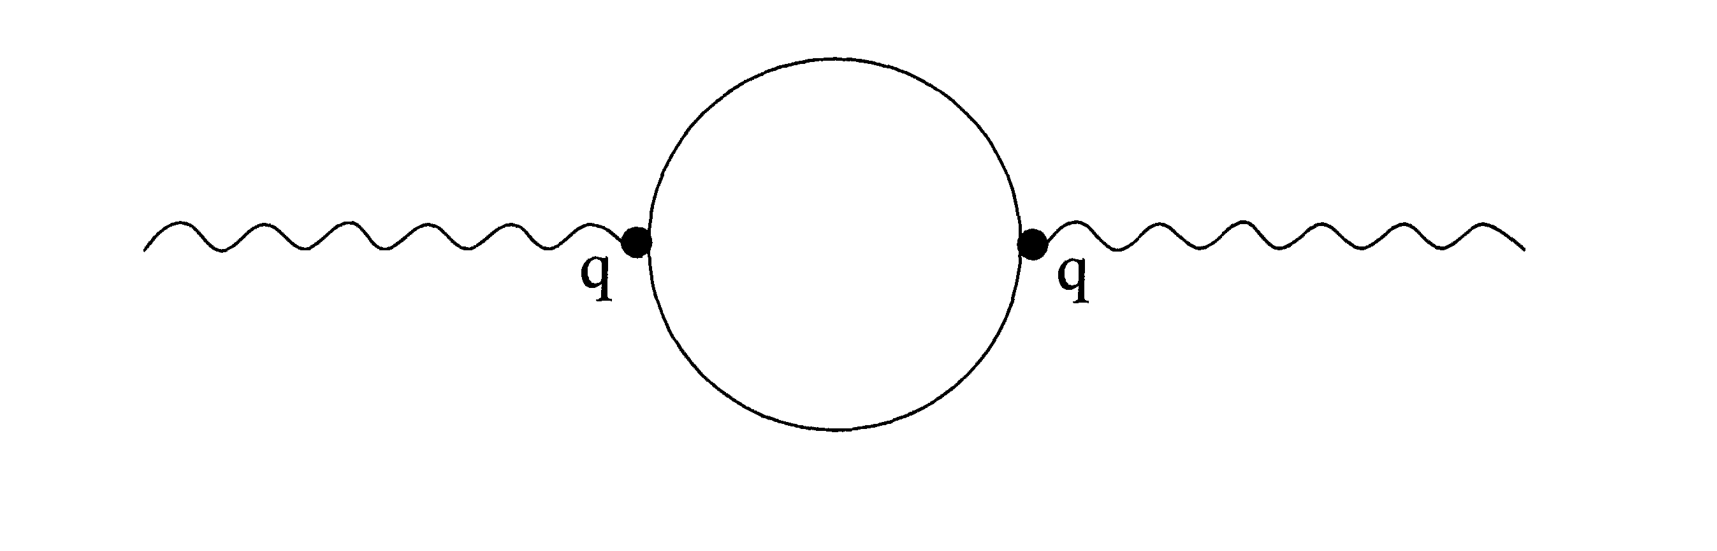
\includegraphics[width=0.62\textwidth]{figs/fig_p254_1.png}
  \caption{规范场（波浪线）经由超多重态（实线）圈的单圈自能图，两侧顶点均标记为荷 $q$。（原文 p.254 的插图，该页未标 Figure 号，此为第 1 张图。）}
  \label{fig:p254-1}
\end{figure}

（实线代表超多重态，波浪线代表矢量多重态。）这张图重整化规范场的动能项；重整化因子是 $u-u_0$ 的函数（因为超多重态的质量正比于 $|u-u_0|$），并且由于超多重态是无质量的，它在 $u\to u_0$ 时按对数发散。

结果是：对 $u$ 靠近 $u_0$ 的情形，我们有

\[
  \tau(u)=2q^2\,\frac{\ln(u-u_0)+\text{constant}}{2\pi i}.
\]

这意味着 $\tau(u)$ 在 $PSL(2,\mathbb{Z})$ 中绕这个奇点的单值变换（monodromy）是

\begin{equation}
  \tag{18.6}
  \label{eq:18-6}
  \pm\begin{pmatrix}1&2q^2\\0&1\end{pmatrix}.
\end{equation}

当然，单值变换实际上是 $SL(2,\mathbb{Z})$ 中的一个元素，由它在 $PSL(2,\mathbb{Z})$ 中的像只确定到相差一个符号。为了把这个符号定下来，我们作如下论证。$u=u_0$ 附近的物理由一个 $U(1)$ 规范理论描述，其规范场为 $(\tilde A,\tilde a)$，并带有一个在 $u_0$ 处变为无质量的带荷超多重态 $(T,\tilde T)$。因此，Lagrange 量具有规范耦合项再加上一个超势 $q\cdot\tilde aT\tilde T$ 的形式。标量场 $\tilde a$ 是 $u$ 平面上的一个局部坐标，而事实上它通过一个 $ISL(2,\mathbb{Z})$ 变换与无穷远处的 $a,a_D$ 相联系。（这个变换在 $SL(2,\mathbb{Z})$ 中的像，由超多重态 $(T,\tilde T)$ 相对于 $u$ 平面中无穷远处那个 $U(1)$ 的荷 $(n_e,n_m)$ 决定。）由于这个 $U(1)$ 理论在整个这个邻域中（甚至在奇点处）都存在，我们看到：在绕 $u_0$ 的单值变换下，场 $\tilde a$ 回到它自身。这意味着在绕 $u_0$ 的 $SL(2,\mathbb{Z})$ 单值变换下存在一个不变向量，从而表明单值变换正是方程 18.6 所写的那样，并且取正号。

% [Tutor Note: 「存在不变向量」这一步是定符号的关键，但作者没有说明它作用在哪一个向量空间上。准确的说法是：矩阵 $\pm\begin{pmatrix}1&2q^2\\0&1\end{pmatrix}$ 的迹是 $\pm2$；而"$\tilde a$ 原样返回"意味着在以 $(\tilde a_D,\tilde a)$ 为基的表示中，该矩阵的本征值必须是 $+1$（而不是 $-1$），故只能取迹为 $+2$ 的那个符号——整体负号会把本征值从 $(1,1)$ 变成 $(-1,-1)$，不变向量随之消失。另有一个极易出错之处：写成 $\begin{pmatrix}1&2q^2\\0&1\end{pmatrix}$ 时，必须明确它作用在列向量 $(\tilde a_D,\tilde a)^T$ 上（于是 $\tilde a_D\mapsto\tilde a_D+2q^2\tilde a$、$\tilde a\mapsto\tilde a$，即 $\tau\to\tau+2q^2$）；若改用 $(\tilde a,\tilde a_D)^T$ 的次序，$2q^2$ 就应挪到左下角。把次序与符号弄混，会得到 $\tau\to\tau-2q^2$ 从而与 $u$ 平面绕无穷远的 $\tau\to\tau-2$（见 (18.2) 与 (18.3)）在方向上讲不通。]

% [Tutor Note: $\ln(u-u_0)+\text{constant}$ 在量纲上并不合法：对数的宗量必须无量纲，而 $u$ 的量纲是质量的平方。规范写法是 $\ln\frac{u-u_0}{\mu^2}$（$\mu$ 为重整化标度），所谓 "constant" 实际上是 $-\ln\mu^2$ 再加上一个有限常数。这不是排印错误而是习惯写法，但它牵动两件事：(i) 常数项若取虚部，等于重新定义 $\theta$ 角，属于允许的重定义；(ii) 关键在于必须写 $\ln(u-u_0)$ 而不是 $\ln|u-u_0|$——只有前者在绕 $u_0$ 一周时给出 $\ln\to\ln+2\pi i$，从而 $\tau\to\tau+2q^2$，这正是 (18.6) 的来源；写成绝对值就得不到任何单值变换。同理，下面对多个超多重态求和时，每一项的对数分支必须取同一套，否则单值矩阵就不再是 $\begin{pmatrix}1&\sum_i2q_i^2\\0&1\end{pmatrix}$。]

我们可以把这一图像加以推广。假定在 $u_0$ 处有若干个荷为 $q_i$ 的超多重态变为无质量。那么 $\tau$ 的局部形式将是

\[
  \tau=2\sum_i q_i^2\,\frac{\ln(u-u_0)+\text{constant}}{2\pi i}.
\]

% ===== 原文 p.255 =====
而绕 $u_0$ 的单值变换将是

\[
  \begin{pmatrix}1&\sum_i2q_i^2\\0&1\end{pmatrix}.
\]

注意：在一个超多重态正在变为无质量的奇点处，单值变换的迹为 $2$，而无穷远处的单值变换的迹为 $-2$。特别地，这意味着：如果奇点来自无质量的超多重态，那么 $u$ 平面上不可能只有一个奇点。（由奇点之外 $\operatorname{Im}\tau$ 的正性，无论如何都可推出单值群必定是非阿贝尔的，因而奇点不止一个。）

\subsection{$\mathcal{M}$ 中奇点的数目}
% 原文 §18.5：The number of singularities in $\mathcal{M}$

为了理解 $\mathcal{M}$ 中奇点的数目，让我们从微观的 $\mathcal{N}=2$ 超对称 $SU(2)$ 理论出发，通过加上如下形式的微扰把它破缺为一个 $\mathcal{N}=1$ 超对称理论：

\begin{equation}
  \tag{18.7}
  \label{eq:18-7}
  \Delta\mathcal{L}=\int d^4x\,d^2\theta\,mu+\text{c.c},
\end{equation}

其中 $m$ 是复常数。（回忆 $u=\operatorname{Tr}\phi^2$。）正如第 16 讲以及 [II-N=1 Dynamics, §2.2] 中所讨论的，这个理论有两个真空，每一个都有质量间隙（mass gap）并且有禁闭（confinement）。

让我们假定，在量子真空空间的某一点处，有 $t$ 个超多重态变为无质量，比如说荷为 $q_i$ 的 $(T_i,\tilde T_i)$。于是在这点附近，物理由一个超势

\[
  W=\tilde a\Bigl(\sum_i q_iT_iT_i'\Bigr)+mu(\tilde a)
\]

描述，其中和以前一样，$\tilde a$ 是 $u$ 平面上的一个局部参数，并通过一个 $SL(2,\mathbb{Z})$ 变换与无穷远处的 $a,a_D$ 相联系。让我们求出宏观理论中的真空空间。也就是说，我们解出 $dW=0$ 并除以 $\mathbb{C}^*$ 作用。显然，方程 $dW=0$ 等价于

\[
  \tilde aT_i=\tilde aT_i'=0\qquad\text{对一切 }i,
\]

\[
  m\frac{du}{d\tilde a}+\sum_{i=1}^{t}q_iT_i\tilde T_i=0.
\]

若 $t>0$，这就给出一个正维数的真空空间。这是不可能的，因为微观理论只有两个真空。这意味着，在每个奇点处都只有一个超多重态变为无质量。其次，由于 $\frac{du}{d\tilde a}\neq0$，我们从第二个方程看出：当 $m\neq0$ 时，一个真空态满足 $T,\tilde T\neq0$。由第一个方程，这意味着 $\tilde a=0$。由于只有一个超多重态，方程变成

\[
  m\frac{du}{d\tilde a}\Big|_{\tilde a=0}+qT\tilde T=0.
\]

这确定了 $T\tilde T$，于是它在 $\mathbb{C}^*$ 作用之下唯一地确定了真空。由此可见，与这个奇点相联系的是一个唯一的真空。

% [Tutor Note: 这里 $T_iT_i'$ 的撇号与同一句中的 $(T_i,\tilde T_i)$ 记号不一致，而紧接在后的第二个 F 项方程又写成 $q_iT_i\tilde T_i$，可见 $T_i'$ 应为 $\tilde T_i$ 的排印之误（或撇号只是权且表示第二个分量）。译文照原样保留 $T_i'$，读者读作 $\tilde T_i$ 即可。另一处被跳过的是"解 $dW=0$ 并除以 $\mathbb{C}^*$ 作用"：在 $\mathcal{N}=1$ 语言中，真空应由 F 项方程 $\partial W/\partial\phi=0$ 与 D 项方程共同决定，再商去复化规范群；此处 $W$ 对 $T_i,\tilde T_i$ 是双线性的、对 $\tilde a$ 是线性的，D 项方程（形如 $\sum_iq_i(|T_i|^2-|\tilde T_i|^2)=0$）总可以沿 $\mathbb{C}^*$ 轨道取到满足，故真空模空间恰为 $\{dW=0\}/\mathbb{C}^*$。这是 Affleck--Dine--Seiberg 关于平直方向（flat direction）的标准论证，可参 Wess--Bagger《Supersymmetry and Supergravity》有关 F/D 平坦性的章节。]

% [Tutor Note: "若 $t>0$ 就得到正维数的真空空间"一句，靠的是：当 $t\geq2$ 时 $\tilde a=0$ 与 $\sum_iq_iT_i\tilde T_i=0$ 只给出一条方程，其余 $2t-1$ 个复方向都是平直的；商去 $\mathbb{C}^*$ 之后仍有 $2t-2>0$ 维，与"微观理论只有两个真空"直接矛盾。这一条正是本节数奇点的全部力量所在，它把 $t$ 硬压到 $1$，从而"一个奇点对应一个真空"。注意 $t=1$ 时方程 $\tilde aT=\tilde a\tilde T=0$ 与 $m\,du/d\tilde a+qT\tilde T=0$ 联立后给出 $\tilde a=0$ 与 $T\tilde T=-m\,du/d\tilde a|_{\tilde a=0}/q$，后者只定出乘积，剩下的相位被 $\mathbb{C}^*$ 吃掉——所以说"唯一确定"。作者没有提 D 项，理由同上一条批注。]

% ===== 原文 p.256 =====
宏观理论中每个奇点有一个真空，而微观理论只有两个真空，由此推出 $\mathcal{M}$ 中至多有两个奇点。于是我们看到

\[
  N_h\le2,
\]

其中 $N_h$ 是超多重态变为无质量的那些点的数目。

正如我们已经注意到的，绕一个超多重态无质量之点的单值变换，与无穷远处的单值变换的迹相反，因而它们在 $SL(2,\mathbb{Z})$ 中不是共轭的。所以根据这一点（或者因为我们需要非阿贝尔的单值群才能得到 $\operatorname{Im}\tau>0$），至少必须有两个超多重态变为无质量之点；也就是说 $N_h\ge2$。于是我们得出结论：$N_h=2$。

这样，尽管我们发现 $\mathcal{M}$ 与经典的真空模空间相同，二者却有重要的差别。经典地，$u$ 平面上只有一个奇点；在那里一个非阿贝尔规范群被恢复，但单值变换是阿贝尔的。量子力学地，$u$ 平面有两个奇点；单值变换是非阿贝尔的，但人们在长距离上永远不会遇到未破缺的非阿贝尔规范对称群。量子理论的非阿贝尔单值变换意味着：与经典情形不同，量子真空空间之上的那族环面并不具有常数 $j$ 不变量。这一点从关于 $u=\infty$ 附近行为的渐近公式 (18.2) 就已经清楚了。

到目前为止，我们已经在 $u$ 平面上找到两个奇点，当我们加上方程 18.7 中的微扰时，每个奇点贡献一个真空。既然受微扰的理论中至多有两个真空，由此推出：原来的 $\mathcal{N}=2$ 理论的量子真空空间不可能含有孤立点；因为那些孤立点也会产生受微扰理论的量子真空。这就补上了我们 §18.2 中把 $\mathcal{M}$ 等同于 $u$ 平面这一论证的一处缺口。

我们回忆：量子力学地，经典 Lagrange 量的 $U(1)_R$ 对称性被破缺为 $\mathbb{Z}/8\mathbb{Z}$ 对称性。由于 $u$ 在 $U(1)_R$ 之下荷为四，这个对称性在 $u$ 平面上作为一个 $\mathbb{Z}/2\mathbb{Z}$ 对称性作用。它就是对称性 $u\mapsto-u$。$\mathcal{M}$ 中的两个奇点必须构成一个 $\mathbb{Z}/2\mathbb{Z}$ 轨道，所以它们是点 $\pm u_0$，其中 $u_0\neq0$。正如我们已经看到的，量纲分析告诉我们 $u$ 的量级为 $\Lambda^2$，即理论中质量参数的平方。这意味着我们可以这样选取质量参数 $\Lambda$：使以 $\Lambda$ 标记的量子理论恰好在 $u=\pm\Lambda^2$ 处有奇点。这样我们就采用了引言中所许诺的质量标度参数 $\Lambda$ 的精确定义。注意这个 $\Lambda$ 的选取与我们此前一直使用的选取不同。这一改变的唯一效果，不过是改变公式 18.1 至 18.5 中的常数。

\subsection{新的无质量粒子}
% 原文 §18.6：The new massless particles

下一步是确定究竟是什么在变为无质量。设在一个使无穷远处的单值变换为上三角的基中，在 $\Lambda^2$ 处变为无质量的超多重态的荷为 $(n_e,n_m)$。若 $n_m=0$，则 $\Lambda^2$ 处的单值变换与无穷远处的单值变换对易。由于该族非奇异部分的全空间（total space）是三孔球面，$\Lambda^2$ 处与 $\infty$ 处的单值变换生成整个单值像。于是，如果 $\infty$ 处与 $\Lambda^2$ 处的单值变换同时为上三角，那么整个单值像都是上三角的，从而是可交换的。这将意味着 $\operatorname{Im}\tau$ 不可能处处为正。我们的结论是 $n_m\neq0$。也就是说，这个粒子……

% [Tutor Note: "该族非奇异部分的全空间（total space）是三孔球面"一语按字面读，维数就不对：族的全空间是椭圆纤维化的复曲面（复维数二），而只有底空间——即 $u$ 平面去掉 $+\Lambda^2,-\Lambda^2,\infty$ 三点，也就是 $\mathbb{CP}^1$ 去掉三点——才是三孔球面。此处 total space 应读作"底空间（base）"。这一点关系到下一句的逻辑：单值表示是底空间基本群的表示，而三孔球面的 $\pi_1$ 是秩二的自由群（绕其中两个 puncture 的圈即可生成，第三个是二者的乘积），所以"$\Lambda^2$ 处与 $\infty$ 处的单值变换生成整个单值像"才成立；若真按全空间理解，基本群还要多出纤维（环面）的两条圈，结论就不对了。]

% ===== 原文 p.257 =====
……在 $u=\Lambda^2$ 处变为无质量，因而带磁荷。对 $-\Lambda^2$ 处的奇点，完全相同的分析成立。这是一个非常有趣的现象。那些在 $|u|\gg\Lambda^2$ 时作为有质量孤子而开始其生命的粒子，随着 $u$ 趋近 $\pm\Lambda^2$ 而变为无质量。这也意味着，我们把 $\pm\Lambda^2$ 附近的理论描述为一个 $U(1)$ 理论，与 $u$ 平面中无穷远附近理论的 $U(1)$ 表示是不同的表示。

现在我们要计算这些粒子的磁荷 $\pm n_m$。注意：当我们从无穷远走入时，$\pm n_m$ 是良定义的，与我们从无穷远到 $\pm\Lambda^2$ 所选取的路径无关；但电荷却依赖于路径——如果我们绕这一对奇点转一圈，$\pm n_e$ 会改变两倍的磁荷，因为绕无穷远的单值变换是 $n_e\mapsto-n_e+2n_m$。$u=\infty$ 附近的磁单极子有 $n_m=\pm1$。这强烈地提示：在奇点处变为无质量的超多重态有 $n_m=\pm1$；这是一个重要的论断，我们将在 §18.7 中更精确地论证它。

我们今天讨论的这个模型有各种数学应用，但仅就物理而言，它最引人注目的应用之一是给出了一个关于禁闭的新模型。我们回忆：禁闭是指外加电荷之间存在线性势，或者等价地，在适当的表示中 Wilson 圈按面积律（area law）衰减（在目前的例子中，$SU(2)$ 的二维表示是个好选择）。我们从第 10 讲 §10.3 回忆起，在 Higgs 相中，当一个带荷场获得真空期望值\footnote{这是一个多少不够精确的描述，正如我们在前面几讲中所见，但在弱耦合下是成立的。}时，人们可以用一个拓扑论证显式地算出 't Hooft 圈按面积律衰减。如果人们能够天真地交换电与磁，那么 Wilson 圈就会与 't Hooft 圈互换，我们就会得出结论：一旦一个带磁荷的场获得真空期望值，禁闭就会出现。1970 年代 't Hooft、Mandelstam、Nambu 等人曾以启发性的方式论证过这一点，但在给出实际模型方面困难极大；因为在这个形式体系中通常并没有带磁荷的场，而带磁荷的客体（它们作为经典解出现）在弱耦合区域——正是在那里人们才能具体地理解它们——是很重的。因此，一般很难看出究竟怎样才能真正展示出一个带磁荷的场获得真空期望值的现象。

在目前的背景下，这件事发生了。我们已经看到，在把 $mu$ 微扰加到超势上之后（这一微扰预期给出禁闭），$u=\Lambda^2$ 附近的真空具有非零的超多重态场 $T,\tilde T$；所以在事实上，在这个真空中（$n_m$ 非零）一个带磁荷的客体已经获得了真空期望值。于是，正如所预期的，恰好在禁闭的情形中一个带磁荷的场获得了真空期望值。为了更精确地追踪这一点，所讨论的带磁荷的场具有奇数 $n_m$ 是重要的。的确，由于 $SU(2)$ 的中心是 $\mathbb{Z}/2\mathbb{Z}$，通过通常 Higgs 机制的对偶来解释禁闭，要求奇 $n_m$ 的场具有非零的期望值。$T$ 与 $\tilde T$ 实际上有奇数的 $n_m$，事实上就是 $\pm1$，正如我们上面以启发性的方式所论证、并将在 §18.7 中更精确地论证的那样。

已经发生的令人惊讶的事情之一是下面这件事。磁单极子在无穷远处的质量量级为 $\sqrt{|u|}\ln(|u|)$，而另外还有一些质量量级为 $\sqrt{|u|}$ 的 BPS 态。因此在无穷远处，磁单极子并不是……

% [Tutor Note: 这一段是全书最值得停下来想的一处对照。作者先说"如果能够天真地交换电与磁"——请注意这只是形式上的互换，不是任何对称性：电、磁的耦合常数互为倒数，弱耦合的磁图像正对应强耦合的电图像，所以这条推理只能算启发式的。真正的定量条件是：禁闭是关于 $SU(2)$ 的中心 $\mathbb{Z}/2\mathbb{Z}$ 的陈述（基本表示的 Wilson 圈只依赖 $n_e\bmod2$），对偶的 Higgs 机制要"探测"到这个中心，凝聚的磁荷就必须是奇数，$n_m\equiv1\pmod2$；若 $n_m$ 为偶数，凝聚对中心是"透明"的，磁通管可以被屏蔽，得不到面积律。另请注意"通常并没有带磁荷的场"这句话的准确含义：拉格朗日量里没有基本场携带 $n_m\neq0$，磁荷只能作为经典解（孤子）出现，因此磁荷凝聚必然是**非微扰**效应——这正是本模型在 1994 年显得惊人的原因。最后，"第 10 讲 §10.3"这一处引文在原文中印作 "Lecture 10.3"，与 p.260 参考文献里"第 10 讲"的说法对照，应读作第 10 讲的 §10.3（即该讲第 3 节），而不是"第 10.3 讲"。]

% ===== 原文 p.258 =====
……有质量粒子中最轻的。然而，在奇点处变为无质量的恰恰就是它们。在这一段里，我们实际上跑到了故事的前面，假定了在奇点处变为无质量的粒子，就是人们在大的 $|u|$ 处半经典地看到的那些 BPS 磁单极子。

\subsection{椭圆曲线族的显式性质}
% 原文 §18.7：Explicit nature of the family of elliptic curves

现在我们准备把各部分拼起来并求解这个模型。我们将显式地描述与本理论量子真空空间相联系的椭圆曲线族以及二形式 $\eta$。正如我们已经看到的，对这个理论而言，量子真空的模空间是 $\mathbb{C}$，参数为 $u=\operatorname{Tr}\phi^2$。该族在无穷远处的 $SL(2,\mathbb{Z})$ 单值变换是

\[
  \begin{pmatrix}-1&2\\0&-1\end{pmatrix}.
\]

此外，$u$ 平面上还有另外两个奇点 $\pm\Lambda^2$。在每个这样的点处，$SL(2,\mathbb{Z})$ 单值变换 $m_{\pm\Lambda^2}$ 的迹为二。我们写

\[
  m_{\Lambda^2}^{-1}=\begin{pmatrix}1+b&-b^2/a\\ a&1-b\end{pmatrix},
\]

其中 $a,b$ 为整数。（这是迹为二、行列式为一的矩阵的一般形式。）由于

\[
  m_{-\Lambda^2}=m_{\Lambda^2}^{-1}m_\infty
\]

的迹为二，我们推出

\[
  2=\operatorname{Tr}\begin{pmatrix}1+b&-b^2/a\\ a&1-b\end{pmatrix}\begin{pmatrix}-1&2\\0&-1\end{pmatrix}.
\]

由直接计算可得 $a=2$。由于 $-b^2/a$ 是整数，我们看到 $b$ 是偶数。现在让我们用矩阵

\[
  \begin{pmatrix}1&1\\0&1\end{pmatrix}
\]

来共轭 $m_{\Lambda^2}^{-1}$ 的矩阵，这个矩阵与无穷远处的单值变换对易。其效果是把 $b$ 改变 $2$。于是，经过若干次这样的共轭之后，我们到达 $b=0$。这意味着，在适当的基下，无穷远处的单值变换是

\[
  \begin{pmatrix}-1&2\\0&-1\end{pmatrix},
\]

而在 $\Lambda^2$ 处的单值变换具有形式

\[
  \begin{pmatrix}1&0\\-2&1\end{pmatrix}.
\]

这样，我们就证明了单值表示在 $SL(2,\mathbb{Z})$ 中唯一地确定到共轭。还要注意，按照方程 18.6，为了得到这个单值变换，在 $\Lambda^2$ 处变为无质量的超多重态的磁荷 $n_m$ 是 $\pm1$。当然，在 $-\Lambda^2$ 处同样成立。事实上，由于 $SL(2,\mathbb{Z})$ 表示唯一地确定到共轭，它在对称性 $u\mapsto-u$ 之下（在共轭的意义下）是不变的。

很容易识别出在上述单值变换下、两度穿孔平面之上的椭圆曲线族。该族的底空间可以等同于模曲线 $\mathbb{H}/\Gamma(2)$，它由把上半平面除以……

% [Tutor Note: "由直接计算可得 $a=2$"这一步值得完整写出，它是本页唯一的硬计算。把两矩阵相乘：$(1,1)$ 元为 $(1+b)(-1)+(-b^2/a)\cdot0=-1-b$；$(1,2)$ 元为 $(1+b)\cdot2+(-b^2/a)(-1)=2+2b+b^2/a$；$(2,1)$ 元为 $a\cdot(-1)+(1-b)\cdot0=-a$；$(2,2)$ 元为 $a\cdot2+(1-b)(-1)=2a-1+b$。故迹为 $(-1-b)+(2a-1+b)=2a-2$，令其等于 $2$ 即得 $a=2$——注意 $b$ 恰好消掉，这正是这个 ansatz 的用意。随后"$b$ 是偶数"用的是 $-b^2/a=-b^2/2\in\mathbb{Z}\Rightarrow b^2$ 偶 $\Rightarrow b$ 偶。最后一步共轭之所以"只改变 $b$ 而不改变 $m_\infty$"，是因为 $\begin{pmatrix}1&1\\0&1\end{pmatrix}$ 与 $m_\infty=\begin{pmatrix}-1&2\\0&-1\end{pmatrix}$ 对易（后者等于 $-T^{-2}$，与 $T$ 生成同一个抛物子群）；若误用 $\begin{pmatrix}1&0\\1&1\end{pmatrix}$ 之类不同矩阵去共轭，$m_\infty$ 会变形，整个论证就失效了。]

% [Tutor Note: 顺带验证一下记号的自洽性：形如 $M(a,b)=\begin{pmatrix}1+b&-b^2/a\\a&1-b\end{pmatrix}$ 的矩阵行列式恒为 $(1+b)(1-b)+b^2=1$，其逆为 $\begin{pmatrix}1-b&b^2/a\\-a&1+b\end{pmatrix}=M(-a,-b)$，仍属同一族。所以作者把 $m_{\Lambda^2}^{-1}$ 而非 $m_{\Lambda^2}$ 写成这个一般形，在迹方程里并不引入额外内容（$a\to-a$、$b\to-b$ 不过是重新命名整数参数）；真正要紧的是 $m_{-\Lambda^2}=m_{\Lambda^2}^{-1}m_\infty$ 中两个因子的次序，它由基的选取（先绕 $\Lambda^2$、再绕 $\infty$ 的合成顺序）决定——两个抛物元不交换，把次序颠倒通常会得到另一个解。判断次序是否正确的办法：解出的矩阵必须与 (18.6) 的 $\begin{pmatrix}1&2q^2\\0&1\end{pmatrix}$（$q=\pm1$）共轭，也就是迹为 $+2$ 且与 $m_\infty$ 一起生成非阿贝尔群；若解出的 $m_{\Lambda^2}$ 迹为 $-2$，说明次序或符号搞反了。]

% ===== 原文 p.259 =====
……$PSL(2,\mathbb{Z})$ 中由所有模二同余于恒等元的矩阵构成的子群的（自由）作用而得到。该族就是这个底空间上具有"二阶结构"（level two structure）的椭圆曲线万有族（universal family）。由于奇点在 $u=\pm\Lambda^2$ 处，与这个量子理论相联系的椭圆曲线族的 Weierstrass 方程是

\[
  y^2=(x-u)(x-\Lambda^2)(x+\Lambda^2).
\]

现在让我们考虑上一讲中所描述的二形式 $\eta$。我们知道，在上面给出的 Weierstrass 模型中，$\eta$ 具有一般形式

\[
  \eta=f(u)\,du\,\frac{dx}{y}.
\]

隐含地，在以前的讨论中我们假定了 $\eta$ 是一个没有零点与极点的复辛形式，至少远离 $u$ 的例外值。这样的零点或极点会产生非物理的奇点。如果我们取 $f$ 为非零常数，那么 Kähler 形式 $\pi_*(\eta\wedge\bar\eta)$ 除在 $\infty,\pm\Lambda^2$ 之外是光滑的，而在那里它具有正确的奇异行为。任何别的 $f$ 都会在别处产生极点或零点，或者在 $\infty,\pm\Lambda^2$ 之一处产生错误的奇异行为。由此推出：对某个适当的常数 $C$ 有 $\eta=C\,du\,\frac{dx}{y}$；这个常数可以通过与 $u=\infty$ 附近 $a^2=u$ 的公式相比较而算出。

显然，

\[
  \eta=d\Bigl(C\frac{u\,dx}{y}\Bigr)=d\Bigl(C\frac{2y\,dx}{x^2-\Lambda^4}\Bigr).
\]

形式 $\lambda=2Cy\,dx/(x^2-\Lambda^4)$ 是椭圆曲线族全空间 $\mathcal{E}$ 上的一个第二类微分（differential of the second kind）。这意味着——正如我们一直所断言的那样——$[\eta]\in H^2(\mathcal{E};\mathbb{C})$ 是平凡的，从而我们这个理论表示族的单值变换包含在 $SL(2,\mathbb{Z})$ 之中，即在更大的群 $ISL(2,\mathbb{Z})$ 之内。这是意料之中的，因为除了 $n_e,n_m$ 之外这个理论没有守恒荷。

% [Tutor Note: 这一串等号值得自己验算，因为"$[\eta]=0$"这一结论完全压在它上面。在总空间上以 $(u,x)$ 为局部坐标（$y$ 由 $y^2=(x-u)(x^2-\Lambda^4)$ 决定，故 $y_u=-(x^2-\Lambda^4)/(2y)$，从而 $d(dx/y)=d(1/y)\wedge dx=-y_u\,du\wedge dx/y^2$），有
% $d\bigl(u\frac{dx}{y}\bigr)=\frac{du\wedge dx}{y}\Bigl[1+\frac{u(x^2-\Lambda^4)}{2y^2}\Bigr]=\frac{2x-u}{2(x-u)}\cdot\frac{du\wedge dx}{y}$，
% 一般不等于 $\eta=C\,du\wedge dx/y$；而
% $d\bigl(\frac{2y\,dx}{x^2-\Lambda^4}\bigr)=\frac{2y_u\,du\wedge dx}{x^2-\Lambda^4}=-\frac{du\wedge dx}{y}$，
% 与 $\eta$ 只差一个整体符号（可并入常数 $C$ 的符号，或等价地把 $\lambda$ 定义为 $-2Cy\,dx/(x^2-\Lambda^4)$）。所以印刷的这条链式等式里，第二个等号只差符号（无害），第一个等号则差一个依赖 $u,x$ 的因子 $\frac{2x-u}{2(x-u)}$（例如在 $x=3,\ \Lambda=1,\ y=2$ 处该因子为 $7/2$），疑为笔误。幸而"$\eta$ 恰当、从而 $[\eta]=0$"只需第二个等号（至多差符号），结论不受影响。引用时请以显式计算为准。]
%
% [Tutor Note: "第二类微分"与"$[\eta]$ 平凡"之间的推理容易被误读成后者是前者的定义性推论。准确的说法是：第二类微分指留数全为零的亚纯微分；留数为零保证 $\lambda$ 沿围绕任何极点的闭路积分不产生 $2\pi i$ 型的多值性，于是 $\lambda$ 是 $\mathcal{E}$ 上单值良定义的 $1$-形式，$\eta=d\lambda$ 便是整体恰当的，这才给出 $[\eta]=0\in H^2(\mathcal{E};\mathbb{C})$，并且 $\eta$ 沿闭链的周期可由 $\lambda$ 的周期直接读出（这正是确定 $a,a_D$ 的基础）。反之，若 $\lambda$ 在某处有非零留数（例如沿一条退化纤维），$\eta$ 就只能在该除子的补集上恰当，$[\eta]\neq0$，单值群便会落在 $ISL(2,\mathbb{Z})$ 而不在 $SL(2,\mathbb{Z})$ 中——这正是作者紧接着要排除的情形。]

\subsection{BPS 谱的描述}
% 原文 §18.8：Description of the BPS spectrum

通过对我们已经找到的椭圆曲线族作进一步研究，可以证明：$u$ 平面中 $a/a_D$ 为实的曲线是一条简单闭曲线，它经过点 $u=\pm\Lambda^2$，并且与实 $u$ 轴再无其他交点。在这条闭曲线之外，BPS 谱是连续的。从 $u=\infty$ 出发趋近，我们看到在 $u=\Lambda^2$ 处有 $a_D=0$ 而 $a\neq0$，而在 $u=-\Lambda^2$ 处有 $-a+a_D=0$ 而 $a\neq0$。（当然，确切的值依赖于从 $\infty$ 到 $\pm\Lambda^2$ 所选的路径，但如果我们沿正实轴或负实轴从无穷远走入，上述方程成立。）由于我们可以从无穷远趋近这两个奇点而不穿过 BPS 态的跳变轨迹（jumping locus），我们看到：在 $u=\pm\Lambda^2$ 处变为无质量的 BPS 态，确实就在无穷远处的原有 BPS 态之中。也就是说，这些粒子是无穷远处原有磁单极子的解析延拓。这就证实了早先以不那么正式的方式所提示的东西。

现在让我们考察：在跳变轨迹上除 $\pm\Lambda^2$ 之外的其他点处，是否还有被迫变为无质量的粒子。当我们沿跳变线在从 $\Lambda^2$ 到 $-\Lambda^2$ 的开上半弧上移动时，我们发现对每个满足 $0<s<1$ 的 $s$，都存在一个使 $sa-a_D=0$ 的点。因此，如果在无穷远处有一个 BPS 态，其荷 $(n_e,n_m)$ 对某个 $t\in\mathbb{R}$ 满足 $(n_e,n_m)=t(s,-1)$，那么在……

% ===== 原文 p.260 =====
……这条开弧上的某一点处，我们发现这个态变为无质量。这一点，再加上对跳变线的开下半弧所作的对称论证，表明：无穷远处所有荷 $(n_e,n_m)$ 满足 $0\le|n_e|\le|n_m|$ 的 BPS 态，都在跳变曲线上某处变为无质量（这恰好发生在点 $u=\pm\Lambda^2$ 处，当且仅当 $n_e=0$ 或 $n_e=\pm n_m$）。通过在无穷远处作一次单值变换（对大的 $u$ 而言它是谱的对称性），任何 $n_m\neq0$ 的 BPS 态都可以映到某个满足 $|n_e|\le|n_m|$ 的态。所以，无穷远处每一个 $n_m\neq0$ 的 BPS 态，只要沿适当的围道从无穷远把它引进来，都会在跳变线上某处变为无质量。

由于跳变线上除对应于 $a_D=0$ 或 $a_D-a=0$ 的那些奇点之外没有别的奇点，而由于那些奇点只用一个变为无质量的超多重态来解释，我们得出结论：对大的 $u$ 而言，除了已纳入我们分析的那些 $n_m=\pm1$ 的态之外，没有 $n_m\neq0$ 的 BPS 态。

这个论断蕴涵着关于经典几何的如下陈述。设 $\mathcal{W}_k$ 是本理论 $k$ 单极子解的模空间，再除以平移与整体 $U(1)$ 旋转而约化。它是一个维数为 $4k-4$ 的超 Kähler（hyper-Kähler）流形，在数学上已被大量研究。可以证明：$\mathcal{W}_k$ 上的 $L^2$ 全纯形式（可能取值于一个平坦线丛（flat line bundle））会给出 $k$ 单极子束缚态，$k>1$。这样的束缚态会产生不想要的奇点，或者对奇点处的单值变换作出不想要的贡献，所以 $\mathcal{W}_k$ 上不应有 $L^2$ 全纯形式。更一般地，A. Sen 利用 $\mathcal{N}=4$ 超 Yang--Mills 理论的对偶性（而不是本讲所考虑的 $\mathcal{N}=2$ 理论）所作的一个论证，定出了 $\mathcal{W}_k$ 的完整 $L^2$ 上同调。

% [Tutor Note: "对每个 $s\in(0,1)$ 有 $sa-a_D=0$ 之点"与后文"$0\le|n_e|\le|n_m|$"之间的对应，本质是边缘稳定性（marginal stability）条件：中心荷为 $Z=n_ea+n_ma_D$，代入 $(n_e,n_m)=t(s,-1)$ 得 $Z=t(sa-a_D)$，故"该态在某点变为无质量"（$Z=0$）恰等价于该点满足 $sa=a_D$。$s$ 跑遍 $(0,1)$ 给出荷矢量的一个开锥；端点 $s=0$ 与 $s=1$ 分别对应 $n_e=0$ 与 $n_e=\pm n_m$，也就是奇点 $u=\pm\Lambda^2$ 所在的两个端点——这正是括号里那句"当且仅当"的来源。另注意原文此处印作 "all the BPS states at infinity that satisfy of charges $(n_e,n_m)$ with ..."，"satisfy of charges" 是明显的语病（应为 satisfy 或 have charges），译文按语义译出，不影响内容。]

\subsection{参考文献与交叉引用}
% 原文 References and cross references

正如标题所表明的，本讲建立在第 17 讲的基础之上；和以前一样，基本文献是

N. Seiberg and E. Witten, \emph{Electric--Magnetic duality, monopole condensation,
and confinement in $\mathcal{N}=2$ supersymmetric Yang--Mills theory},
Nucl. Phys. B \textbf{426} (1994), pp. 19--52.

关于 Sen 工作的文献是

A. Sen, \emph{Dyon--Monopole Bound States, Selfdual Harmonic Forms On The
Multi-Monopole Moduli Space, and $SL(2,\mathbb{Z})$ Invariance In String Theory},
Phys. Lett. \textbf{B329} (1994) pp. 217--221.

't Hooft 圈与禁闭在第 10 讲中讨论。单圈 $\beta$ 函数计算的讨论见第 16 讲 §2，也见 [I-Renorm Groups] 的第 2、3 讲以及 [II-CFT] 的第 3 讲。BPS 态在第 12 讲中有详细讨论。

% [Tutor Note: 文献代号 [I-Renorm Groups] 与 [II-CFT] 指本丛书第 I 卷的"重整化群"章与第 II 卷的"共形场论"章（参见本书文献代号表）；本讲的另一文献代号 [II-N=1 Dynamics]（见 p.255）指第 II 卷关于 $\mathcal{N}=1$ 动力学的那一章。这三处代号在原文中一律用方括号大写罗马数字标注，翻译时原样保留，切勿改成书名或页码。]
